\section{Introducción}

La función de Rosenbrock, propuesta originalmente por Howard H. Rosenbrock en 1960, es un referente clásico dentro del ámbito de la 
optimización matemática y computacional. Su relevancia viene en la complejidad de su paisaje de búsqueda: una superficie continua, suave 
y no convexa, caracterizada por un estrecho valle curvado que conduce al mínimo global. 
Esta estructura la convierte en un ejercicio ideal para evaluar el desempeño y la estabilidad de algoritmos de optimización, 
especialmente aquellos inspirados en procesos evolutivos o heurísticos como es nuestro caso.

En este caso abordaremos la función de Rosenbrock con el fin de obtener su mínimo y máximo, además de analizar la capacidad de los métodos 
para escapar de regiones de estancamiento y converger hacia soluciones óptimas en espacios con topologías complejas. 

El enfoque adoptado se centra en una implementación capaz de aproximar el mínimo global de la función 
mediante estrategias adaptativas de selección y mutación. Esta aproximación nos beneficia debido a su naturaleza 
estocástica, que permite un equilibrio entre exploración y explotación del espacio de búsqueda, fomentando la diversidad poblacional. 
De este modo, la optimización de una función de prueba tan exigente como la de Rosenbrock constituye un escenario idóneo para examinar 
la robustez, convergencia y comportamiento dinámico del algoritmo propuesto.
La función de Rosenbrock en dos dimensiones se define matemáticamente como:
\begin{equation}
f(x, y) = {(a - x)}^2 + b{(y - x^2)}^2
\end{equation}
donde \(a\) y \(b\) son parámetros que determinan la forma del valle, siendo comúnmente \(a = 1\) y \(b = 100\). 
El mínimo global de esta función se encuentra en el punto \((x, y) = (a, a^2)\).

En esta ocacion usaremos la función acotada en el rango \([-5, 10]\) para ambas variables \(x\) y \(y\), por lo que nuestra función queda de la siguiente manera:

\begin{figure}[H]
    \centering
    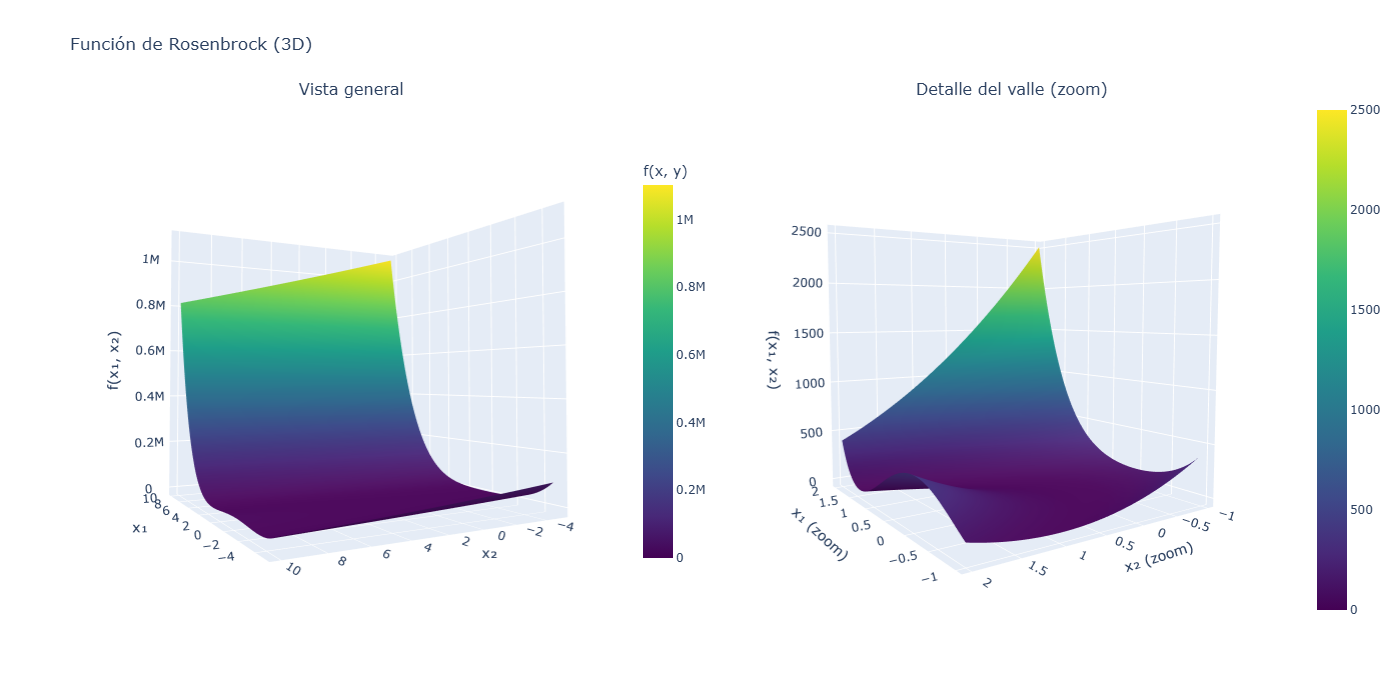
\includegraphics[width=1\textwidth]{rsc/img/intro/rosenbrock.png}
    \caption{Representación gráfica de la función de Rosenbrock en 3D, con zoom en el valle.}\label{fig: funcion}
\end{figure}